\section {Конструкторский раздел}
Для проверки работоспособности схемы необходимо собрать статистически значимое число образцов. 
VirusShare \cite{VIRUSSHARE} предоставляет доступ к коллекции вредоносных образцов за 2011-2015, полученных от различных производителей антивирусов, HoneyPot'ов и других источников, собранных в пачки по 65536 штук.
MalShare Project \cite{MALSHARE} предоставляет доступ на скачивание  всего до 1000 образцов из их хранилища в день, однако у них новые образцы появляются практически ежедневно.

В связи с этим, было принято решение о первоначальном сборе данных на пачках из VirusShare (<<тренировочная>> выборка) и последующей проверке обнаружения цепочек на собираемых ежедневно с начала 2016 года образцов из MalShare (<<тестовая>> выборка). В связи с имеющимися в наличии ресурсами представляется возможным прогнать всего порядка 60000 штук, поэтому разделим выборки на 56634 vs 7657 штук.

После сбора логов и преобразования становится возможным проследить некоторые тенденции в собранных данных. Если посмотреть на график \ref{fig:seq_len_hist}, видно, что значительную часть собранных цепочек составляют те, у которых число вызовов 132 и менее. Скорее всего, большая часть из них относится к тем образцам, у которых по тем или иным причинам не удалось собрать достаточно полную картину вызовов, будь то из-за внезапного завершения работы, проблем обнаружения точки входа упакованных образцов, или каким-либо иным. Длина цепочек большей длины приблизительно соответствует по форме нормальному распределению, а при увеличении числа образцов следовало бы ожидать большей схожести.

\begin {figure}[ht]
        \centering
        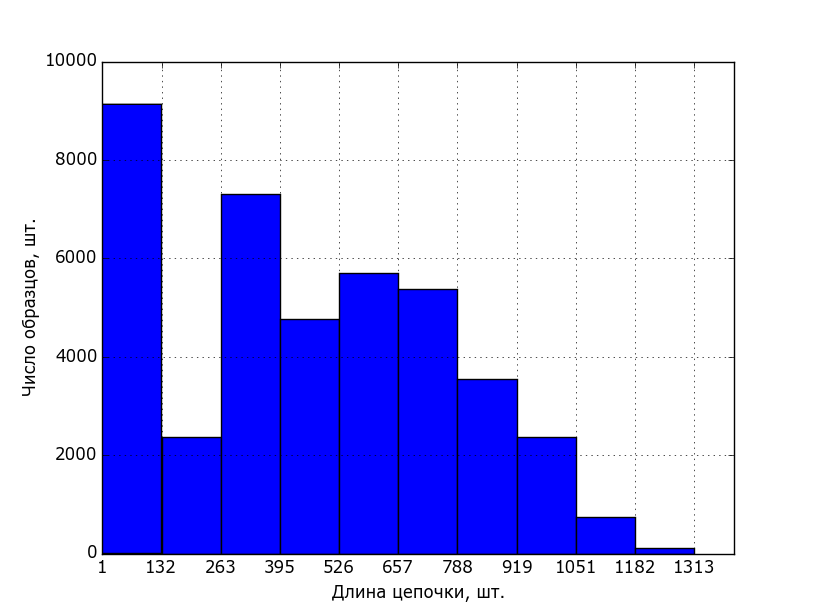
\includegraphics[width=\linewidth] {img/sequence_len_hist.png}
        \caption {Распределение длины цепочек среди образцов}
        \label {fig:seq_len_hist}
\end {figure}

При сравнении цепочек вызовов можно использовать две формы стратегии:
\begin {enumerate}
	\item Быстрая - задание порога, при котором оценка совпадения считается подозрительной. Сравнение с образцами из <<тренировочной>> выборки завершается, как только будет найдено первое подозрительное совпадение, превышающее порог. Это позволяет ускорить сравнение <<тестовой>> выборки. 
	\item Медленная - сравнение с образцами из <<тренировочной>> выборки осуществляется всегда полностью, при этом запоминается максимальные N (например, 3) по оценке совпадения. Это позволяет более точно найти максимально похожие цепочки среди известных, однако сканирование будет занимать максимально возможное время для каждого образца.
\end {enumerate}

Чтобы продемонстрировать возможность обнаружения разных цепочек из одного вируса в других, был выбран один из образцов <<тестовой>> выборки и к нему применена медленная стратегия сравнения. Хэш образца f2b6f4793a2f15ee4fafd95d48d78d55. В результате, одним из похожих найденных образцов <<тренировочной>> выборки является VirusShare\_0002422da43f24e30470fa08f294acbe, который в классификации Dr. Web'а был определён, как Trojan.DownLoad2.19273, другой - VirusShare\_060f15001381480ff0954366c3315d87, который в  классификации Dr. Web'а определяется, как Trojan.Siggen2.22967. Сам же проверяемый образец по той же самой классификации относится к Program.Unwanted.889.


